\documentclass[a4paper, 10pt, oneside, twocolumn, 3p]{elsarticle}

\usepackage{lineno,hyperref}
\usepackage[T1]{fontenc}
\usepackage[utf8]{inputenc}
\usepackage{lmodern}
\usepackage[english]{babel}
\usepackage{graphicx}
\usepackage{float}
\usepackage[siunitx, american, smartlabels, cute inductors, europeanvoltages]{circuitikz}
\usepackage{multirow}
\usepackage{subfig}
\usepackage{amsmath}
\usepackage{mathtools}
\usepackage{enumitem}
\usepackage{rotating}
\usepackage{resizegather}
\usepackage{textgreek}
\usepackage{gensymb}

%% BB
\newcommand{\bb}{\ensuremath{\beta\beta}}
%% BB0NU
\newcommand{\bbonu}{\ensuremath{\beta\beta0\nu}}
%% BB2NU
\newcommand{\bbtnu}{\ensuremath{\beta\beta2\nu}}
%% Qbb
\newcommand{\Qbb}{\ensuremath{Q_{\beta\beta}}}
%% NME
\newcommand{\Monu}{\ensuremath{\Big|M_{0\nu}\Big|}}
\newcommand{\Mtnu}{\ensuremath{\Big|M_{2\nu}\Big|}}
%% PHASE-SPACE FACTOR
\newcommand{\Gonu}{\ensuremath{G_{0\nu}(\Qbb, Z)}}
\newcommand{\Gtnu}{\ensuremath{G_{2\nu}(\Qbb, Z)}}
%% mbb
\newcommand{\mbb}{\ensuremath{m_{\beta\beta}}}
%% BACKGROUND COUNTS
\newcommand{\ckky}{\ensuremath{\rm counts~keV^{-1}~kg^{-1}~y^{-1}}}
%% T0nu
\newcommand{\Tonu}{\ensuremath{T_{1/2}^{0\nu}}}
%% T2nu
\newcommand{\Ttnu}{\ensuremath{T_{1/2}^{2\nu}}}


\newcommand{\cluster}{\emph{cluster}}
\newcommand{\hit}{\emph{hit}}
\newcommand{\hits}{\emph{hits}}
\newcommand{\voxel}{\emph{voxel}}
\newcommand{\voxels}{\emph{voxels}}

%%%%%%%%%%%%%%%%%%%%%%%%%%%%%%%%%%%%%%%%%%%%%%%%%%%%%%%%%%%%

% Xe-136
\newcommand{\CS}{\ensuremath{^{137}}Cs}

% Na22
\newcommand{\NA}{\ensuremath{^{22}}Na}




% Pb-208
\newcommand{\Pb}{\ensuremath{^{208}}Pb}
% Pb-208
\newcommand{\PBD}{\ensuremath{^{210}}Pb}

% Po-214
\newcommand{\Po}{\ensuremath{^{214}}Po}


%%% Ca-48
\newcommand{\CA}{\ensuremath{{}^{48}\rm Ca}}
%%% Ge-76
\newcommand{\GE}{\ensuremath{{}^{76}\rm Ge}}
%%% Se-82
\newcommand{\SE}{\ensuremath{{}^{82}{\rm Se}}}
%%% Zr-96
\newcommand{\ZR}{\ensuremath{{}^{96}{\rm Zr}}}
%%% Mo-100
\newcommand{\MO}{\ensuremath{{}^{100}{\rm Mo}}}
%%% Te-128
\newcommand{\TEI}{\ensuremath{{}^{128}\rm Te}}
%%% Te-130
\newcommand{\TEII}{\ensuremath{{}^{130}\rm Te}}
%%% Nd-150
\newcommand{\ND}{\ensuremath{{}^{150}{\rm Nd}}}
%%% Xe-136
\newcommand{\XE}{\ensuremath{{}^{136}\rm Xe}}
%%% Tl-208
\newcommand{\TL}{\ensuremath{{}^{208}\rm{Tl}}}
%%% Bi-214
\newcommand{\BI}{\ensuremath{^{214}}Bi}

\newcommand{\CO}{\ensuremath{{}^{60}\rm Co}}
\newcommand{\PO}{\ensuremath{{}^{214\rm Po}}}
\newcommand{\U}{\ensuremath{{}^{235}\rm U}}
\newcommand{\CT}{\ensuremath{{}^{10}\rm C}}
\newcommand{\BE}{\ensuremath{{}^{11}\rm Be}}
\newcommand{\BO}{\ensuremath{{}^{8}\rm Be}}
\newcommand{\UDTO}{\ensuremath{{}^{238}\rm U}}
\newcommand{\CD}{\ensuremath{^{116}{\rm Cd}}}
\newcommand{\THO}{\ensuremath{{}^{228}{\rm Th}}}

\newcommand{\RN}{\ensuremath{{}^{222}}Rn}

\modulolinenumbers[5]

\journal{Journal of Nuclear Instruments and Methods in Physics Research Section A}

\bibliographystyle{EP_article}

\begin{document}

\setlength{\parskip}{4mm}
\sloppy \lefthyphenmin=1000

\begin{frontmatter}

\title{NEXT-White experiment energy plane electronics design}

\author[mymainaddress]{Vicente \'Alvarez} \corref{mycorrespondingauthor}
\author[mysecondaryaddress]{Vicente Herrero}
\author[mymainaddress]{Juan Jos\'e Gomez Cadenas} 
\author[mysecondaryaddress]{Ra\'ul Esteve} 
\author[mysecondaryaddress]{Andrew Laing} 
\author[mysecondaryaddress]{Javier Rodríguez} 
\author[mymainaddress]{Marc Querol} 
\author[mysecondaryaddress2]{Francesc Monrabal} 
\author[mysecondaryaddress]{José Francisco Toledo} 
\cortext[mycorrespondingauthor]{Corresponding author (vicente.alvarez@ific.uv.es)}

\address[mymainaddress]{Instituto de Física Corpuscular(IFIC), CSIC \& Universitat de València \\ Calle Catedrático José Beltrán, 2, 46980 Paterna, Valencia, Spain} 
\address[mysecondaryaddress]{Instituto de Instrumentación para Imagen Molecular (I3M), Universtitat Politècnica de València \\ Camino de vera, s/n, Edificio 8B, 46022 Valencia, Spain}
\address[mysecondaryaddress2]{Departament of Physics, University of Texas at Arlington\\ Arlington, Texas 76019, USA}

\begin{abstract}
NEXT-White (NEW) experiment is looking for the neutrinoless double beta decay of  \XE\ , and therefore requires good level of radiopurity. To this end, the PMTs used for the energy measurement and their electronics have been designed and implemented in the NEXT-White (NEW) demonstrator not only considering the 1\% energy resolution required but taking into account radiopurity limitations. The design was done to assure the required front-end electronics specifications such as linearity and low noise and also meet a low radioactivity level. In order to reduce low frequency noise effects and enhance detector's security a grounded cathode connection has been used. A detailed description of the electronics and required signal postprocesing to obtain a liner response and overcome AC coupling effects are provided.

\end{abstract}

\begin{keyword}

 \texttt{Energy, plane  \sep PMT \sep Calometry \sep Front-end electronics \sep FEE  \sep ATCA \sep DSP  \sep BLR}
 

\end{keyword}


\end{frontmatter}

\linenumbers


\section{Introducction}

\par NEXT (Neutrino Experiment with a Xenon TPC) \cite{1748-0221-7-06-T06001} is a neutrinoless double-beta ($\beta\beta 0\nu$) decay experiment at the Canfranc Underground Laboratory (LSC) \cite{LSC}. It seeks to detect the ($\beta\beta 0\nu$) decay of \XE\ using a high pressure xenon gas TPC with electroluminescent (EL) amplification. The NEXT-White (NEW) detector (shown on figure \ref{fig:NEW}), with an active xenon mass of about 10 kg at 15 bar, is the first NEXT prototype installed at Canfranc Underground Laboratory (LSC). It implements the NEXT detector concept tested in smaller prototypes using the same radiopure sensors and materials that will be used in the future  \mbox{NEXT-100}, serving as a benchmark for technical solutions. 

\begin{figure}
  \begin{center}
   	 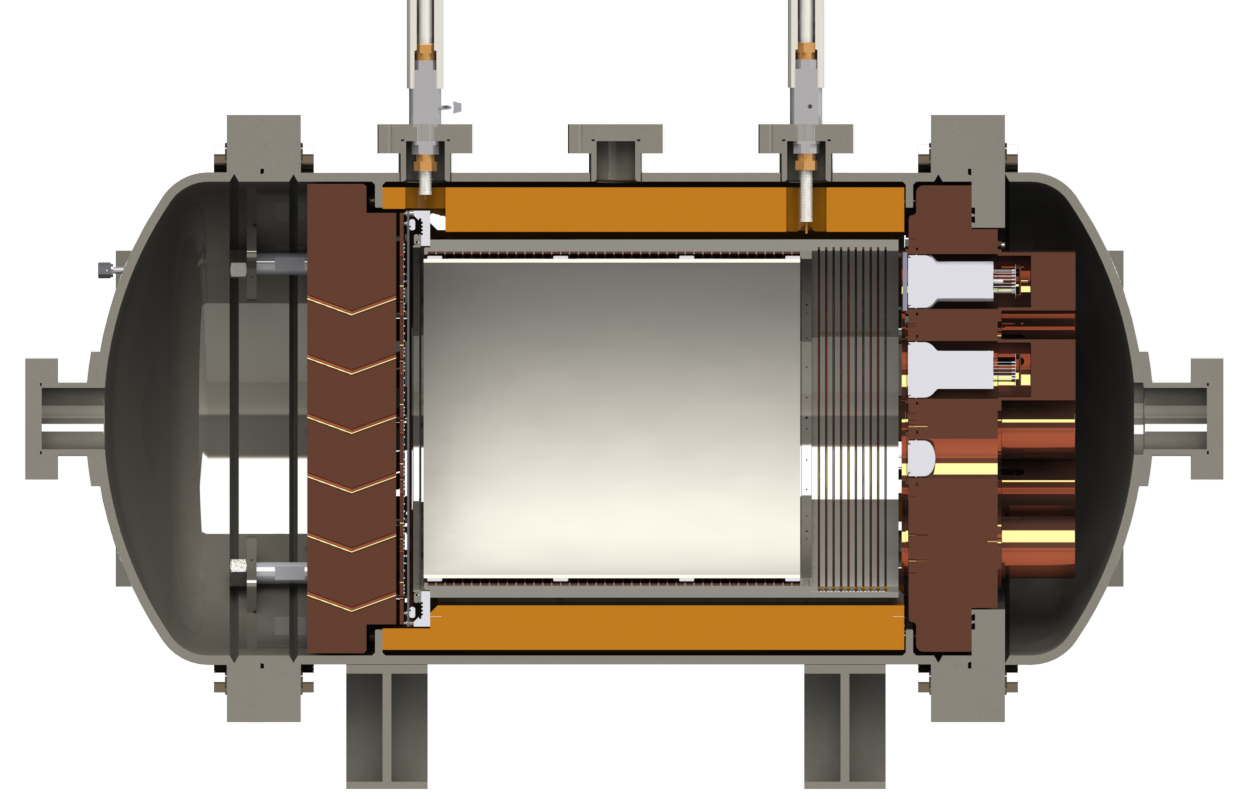
\includegraphics[width=.5\textwidth]{./figures/NEW.png}    
   	 \caption{NEW detector}
   	 \label{fig:NEW}
  \end{center}
\end{figure}

\par The NEW detector is fully operational at LSC. A low background run using depleted Xe is foreseen during 2018; these data will be essential to validate the background model of NEXT-100, based on the radiopurity measurements of all the relevant components.

\par A background of ${4\times10^{-4}}$~\ckky\ in the energy region of interest means the experiment is sensitive to a half life of up to ${6\times10^{25}}$~years after running for 3 effective years \cite{1029-8479,1748-0221-8-01-T01002}. The required background level is achievable thanks to passive shielding, background discrimination techniques based on charged particle tracking \cite{1029-8479,1748-0221-12-01-T01004} and a thorough material radiopurity control. 

\par The energy plane of NEW consists of a 12~cm thick copper support plate with 12 sapphire windows brazed in copper flanges and then screwed to the copper plate (figure \ref{fig:detail}). A 12~cm thick copper cap is placed behind each PMT, to shield the fiducial volume. The energy plane will be held at vacuum levels of less than $10^{-4}$ mbar. The twelve R11410-10 \cite{PMT} PMTs from Hamamatsu are optically coupled to the sapphire windows using NyoGel OCK-451, and held in place with a plastic support and spring. The external face of the windows is coated with tetraphenyl-butadiene (TPB) to shift the xenon VUV light to blue and coated with PDOT (poly(3,4-ethylenedioxythiophene)), a conductive polymer which stops the electric field from the TPC penetrating as far as the PMT dynodes. The twelve PMTs are located 12~cm behind the TPC cathode and cover approximately 30\% of its surface area. This level of coverage was chosen as a compromise between the need to collect as much light as possible and the need to minimize the number of sensors to reduce cost, technical complexity and radioactivity.  The selected model R11410-10 is a 3$"$ PMT specially developed for low-background operation, equipped with a synthetic fused silica window and a photocatode made of low temperature bialkali with high quantum efficiency. 

\par The PMTs receive high voltage and have their signal extracted via kapton twisted cables connected to a feedthrough in the torispherical head of the pressure vessel. The distribution of signal and supply at each individual PMT is done by means of a Kapton circuit board (PMT base) which is covered with a copper cap and filled with epoxy. PMT bases are connected to the support plate to allow generated heat to be dissipated under vacuum conditions.

\begin{figure}
  \begin{center}
   	 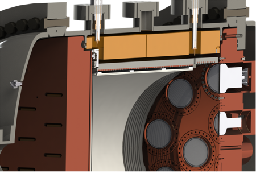
\includegraphics[width=0.5\textwidth]{./figures/EP_detalle.png}   
   	 \caption{Energy plane detail}
   	 \label{fig:detail}
  \end{center}
\end{figure}

The most important design requirement for the energy plane is linearity over the whole dynamic range. In terms of linearity the worst situation is for long signals which could extend for more than 100 microseconds. 



\section {PMT base circuit}

\par PMT bases must meet specifications such as minimum heat dissipation, linearity and low radioactivity. Their design follows the manufacturer reference scheme for grounded cathode connection (fig.~\ref{fig:grounded_cathode}) since the whole detector structure must be connected to earth for electrical safety reasons.

\par Taking into account static power consumption constrains a lower limit for resistor values can be established. Manufacturer recommended ratios between dynodes voltages allow us to define a set of values for base resistors (table \ref{tab:R_C_values}). Total power dissipation for each base circuit depends on the exact high voltage supplied to the PMT and will lie in the range of [30-40]~mW. 

\par PMT base circuit must provide enough charge for the PMT with negligible change in dynode-to-dynode voltage in any situation. Changes in these voltages introduce a time varying gain which acts as a nonlinear distortion mechanism and has a strong effect on PMT linearity. As a consequence in order to provide PMT dynodes with the required charge a certain number of resistor chain stages needs to be backed by capacitors. Table \ref{tab:R_C_values} shows required capacitors as well as their values. 


\begin{table*}[ht]
\scriptsize
	\caption{Resistor \& capacitors base values}
	\label{tab:R_C_values}	
	\begin{center}
		\begin{tabular}{ c | c | c | c | c | c | c | c | c | c | c | c | c | c | c |}
			Dynodes & K & Dy1/G & Dy2 & Dy3 & Dy4 & Dy5 & Dy6 & Dy7 & Dy8 & Dy9 & Dy10 & Dy11 & Dy12 & P\\
			\hline
			Ratio & &  4 & 1.5 & 2 & 1 & 1 & 1 & 1 & 1 & 1 & 1 & 1 & 2 & 1 \\
			\hline
			Resistors & & 8M & 3M & 4M & 2M & 2M & 2M & 2M & 2M & 2M & 2M & 2M & 4M & 4M  \\
			\hline
			Capacitors &  &  &  &  &  &  &  &  &  &  &  & 2x 4,75uF & 3x 1,5uF & 2x 4,75uF  \\
		\end{tabular}
	\end{center}
\end{table*}


\par The capacitors for the base were chosen using the algorithm described in figure \ref{fig:Base_Sizing} where the main goal is to get a worst case drop of 0.1\% in voltage between dynodes. Since each stage increases the gain by a given factor (based on the geometry and characteristics of the PMT) the highest voltage drops will be located at the last stages where the amount of charge to be delivered by the PMT is higher. Therefore starting from the last PMT stage, at least three stages will be backed with capacitors. 

\begin{figure}
  \begin{center}
    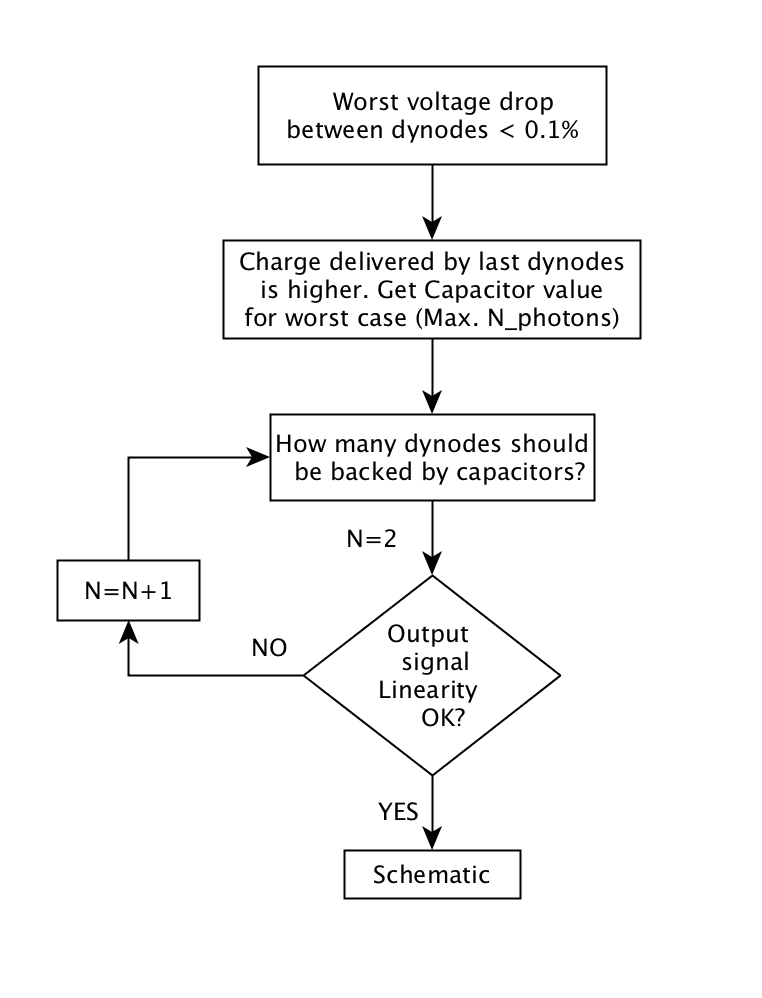
\includegraphics[width=0.45\textwidth]{./figures/diagrama.png}
    \caption{Base Circuit. Capacitor sizing procedure}
    \label{fig:Base_Sizing}
  \end{center}
\end{figure}

\par PMT bias voltage was established through a trade-off between single photon detection capability and manufacturer recommended high voltage (HV) range for best linearity. In order to achieve sufficient SNR, electronics induced noise must be reduced. This imposes a practical limit to the amplifier's gain and demands the use of \mbox{high-gain} PMTs.

% VHB -
%The whole structure must be connected to earth for electrical safety reasons, this fact implies that a PMT grounded cathode connection scheme be used. 

\par In a PMT grounded cathode connection the anode output must be AC coupled through an isolation capacitor since anode output DC voltage equals the high voltage (HV) being applied to the PMT (figure~\ref{fig:grounded_cathode}). As a consequence the AC coupling capacitor must be able to cope with the HV needed to provide the required gain in the PMT (typically from 1000 V to 1750 V). 

\begin{figure} [H]
	\begin{center}
		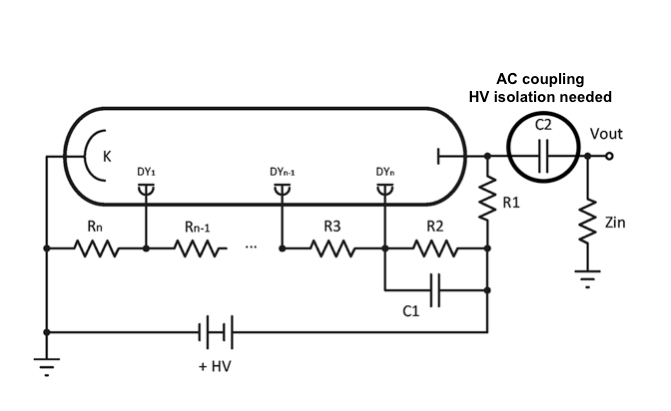
\includegraphics[width=.4\textwidth]{./figures/AC_diagram.png}
		\caption{Grounded Cathode PMT connection scheme}
		\label{fig:grounded_cathode}
	\end{center}
\end{figure}


\par The design is made more challenging due to the required trade-off between radiopurity and linearity. The size and number of components must be carefully studied and limited so that the radioisotope budget is not exceeded without compromising the linearity of the PMT response and, thus, the final energy resolution.



\subsection {Heat dissipation tests}

\par The EP volume can be operated either in vacuum or with N2. For the first case a thermal simulation is mandatory in order to check for possible heat dissipation problems inside the structure.
%For the first case, we needed to know if the heat will be dissipated correctly, wherefore, heat simulation should be done.

\par The maximum expected amount of heat to be dissipated by each base is 40~mW. In order to achieve this in vacuum they will be encased in thermal epoxy (Araldite 2011\textregistered) and connected via a copper cap to the support. Simulations with finite elements software have been carried out and yield a stable operational temperature of 23.6~\degree{C} (figure \ref{fig:temp_simu}) under vacuum condition and ambient temperature of 22~\degree{C}. These results were confirmed in a test bench where a temperature of 24~\degree{C} was achieved with 21~\degree{C} ambient temperature. No disturbances to the rest of the detector are expected with these results. 
 
 
\begin{figure}
  \begin{center}
    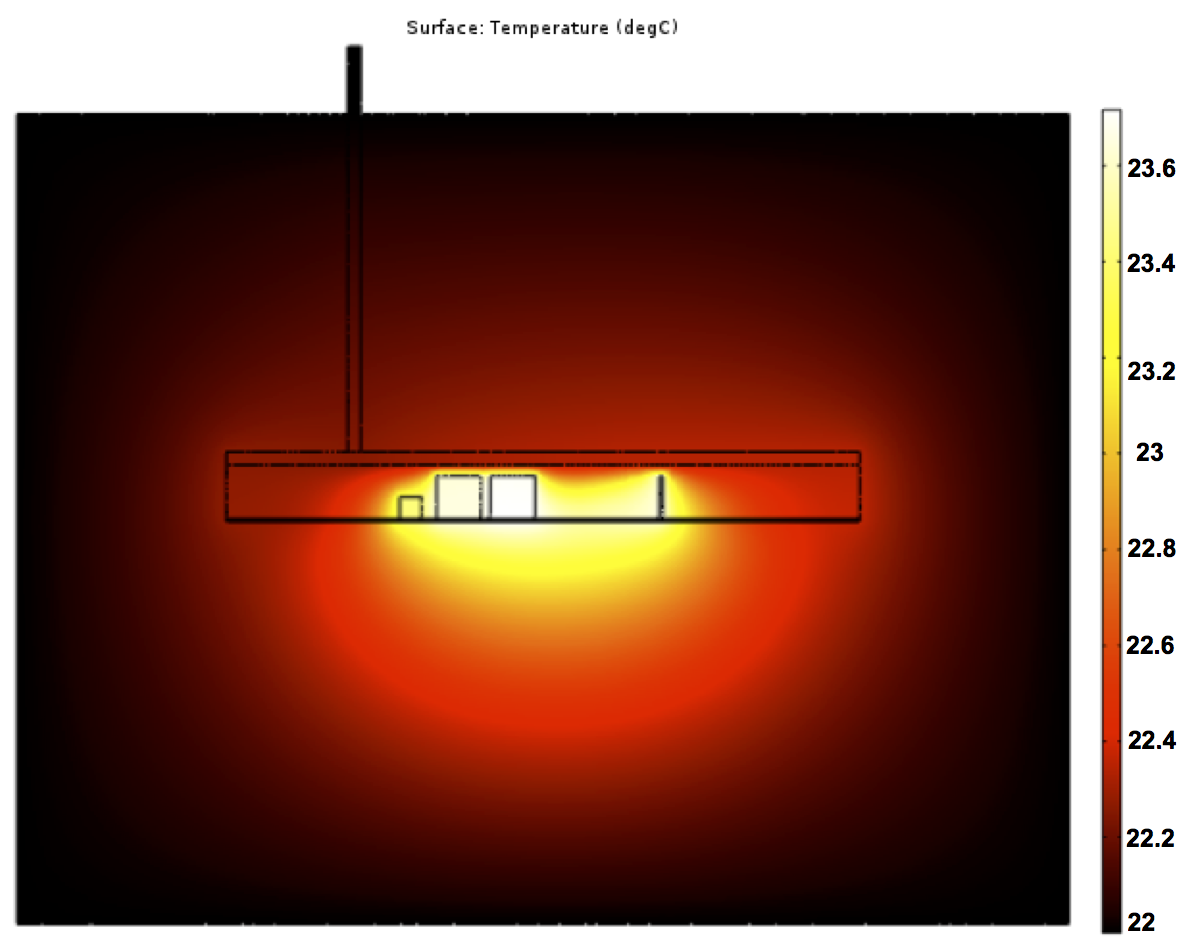
\includegraphics[width=0.4\textwidth]{./figures/temp_simulation.png}
    \caption{Simulation of temperature in Comsol Multiphysics}
    \label{fig:temp_simu}
  \end{center}
\end{figure}

\subsection {Test bench \& linearity measurements}

\par A test bench for linearity measurements was developed in order to test each component under NEW energy plane conditions. The test includes not only a PMT (with its base) but also the associated front-end electronics (FEE) due to the special characteristics of the signals captured and the high linearity required.  The dynamic range of every channel must cover from a single photon up to 100k photons. Moreover, signal length in NEXT can vary from a few microseconds up to $\sim$150~\textmu s which presents an additional challenge to electronics design.

\par The linearity test bench makes use of a signal generator which introduces a voltage square pulse with very short rise and fall edges into the LED (435~nm centered radiation spectrum). The amount of photons being generated is proportional to the length of the pulse. In order to avoid LED switching effects the minimum pulse length is 20~\textmu s (the setting time of the LED is in order of 1~us). The effect of LED output fluctuation is limited by averaging over 200 samples for each device under test. Additionally, a set of 90\% attenuation optical filters were used directly coupled to the LED.

\begin{figure}[H]
	\begin{center}
		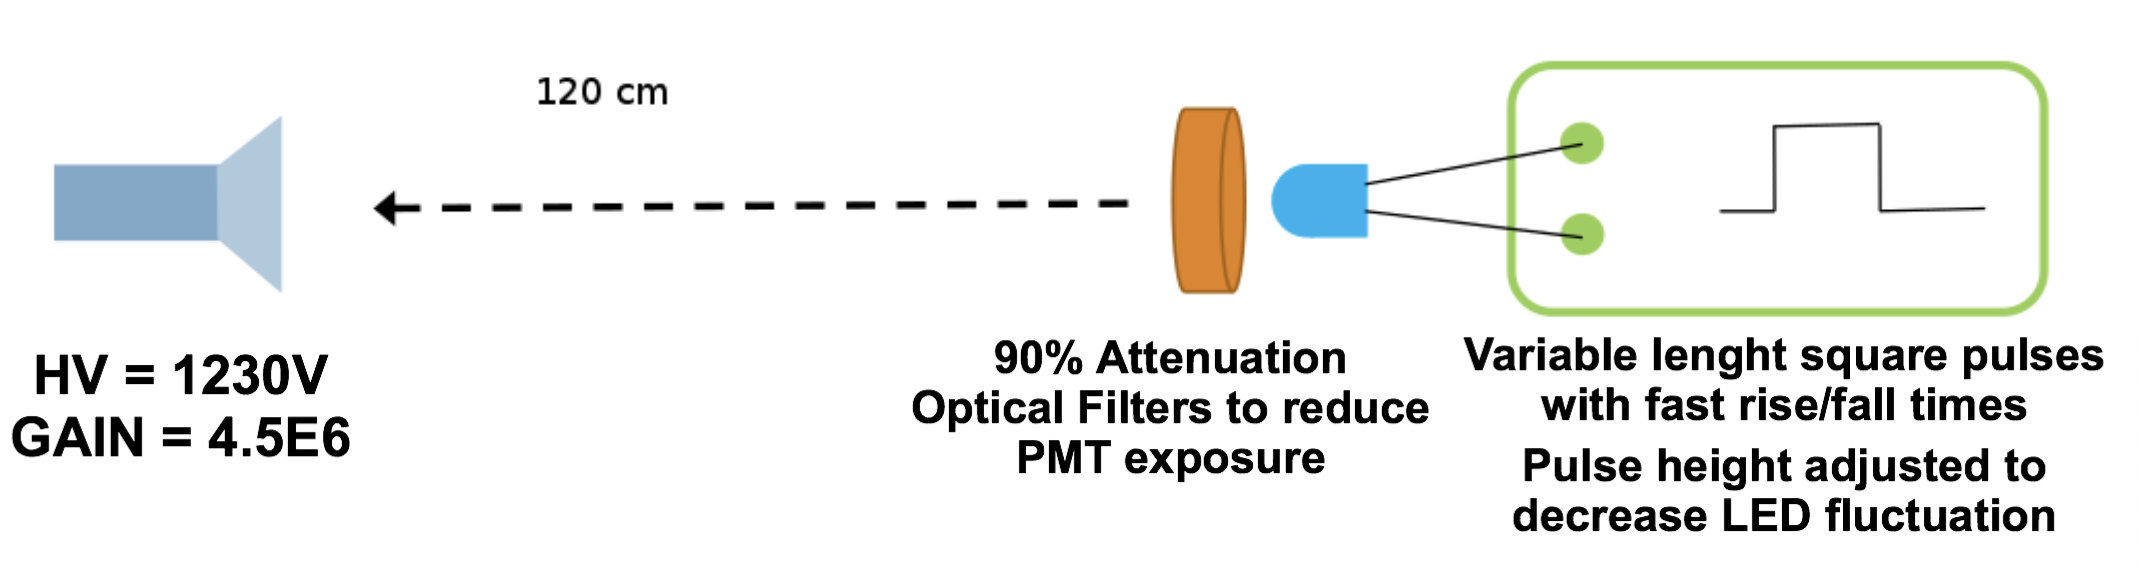
\includegraphics[width=0.5\textwidth]{./figures/LED_testbench1.png}
		\caption{LED based PMT+FEE test bench for linearity measurements}
		\label{fig:LED_testbench}
	\end{center}
\end{figure}


%\begin{figure}
%  \begin{center}
%    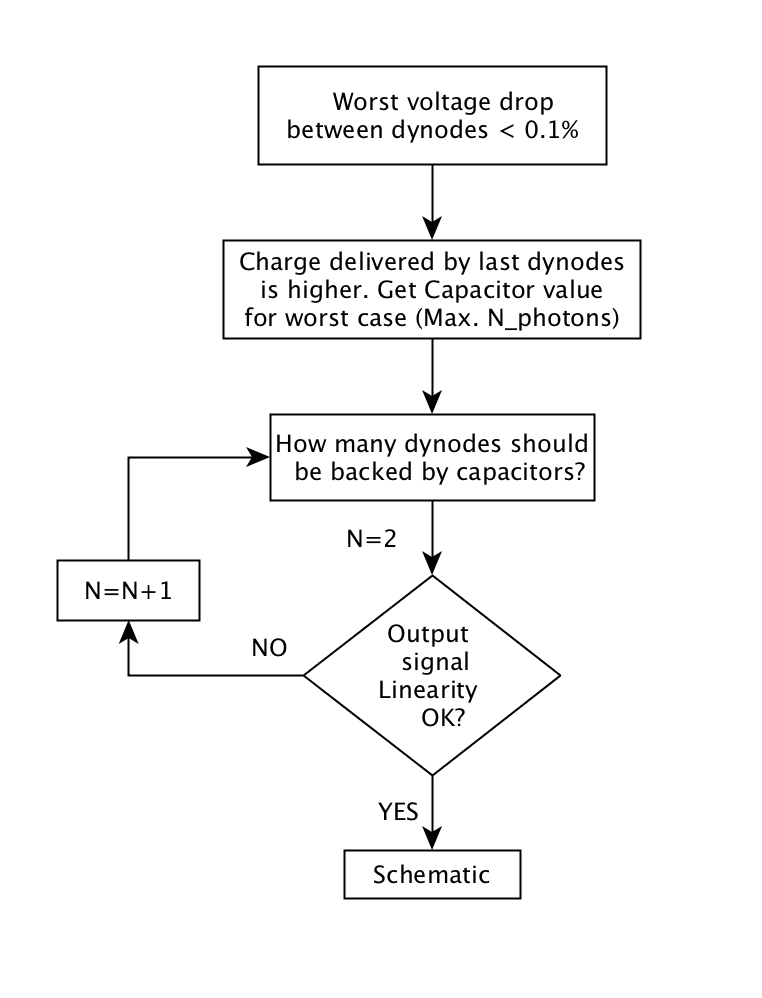
\includegraphics[width=0.45\textwidth]{./figures/diagrama.png}
%    \caption{Base Circuit. Capacitor sizing procedure}
%    \label{fig:Base_Sizing}
%  \end{center}
%\end{figure}


\begin{figure}
  \begin{center}
    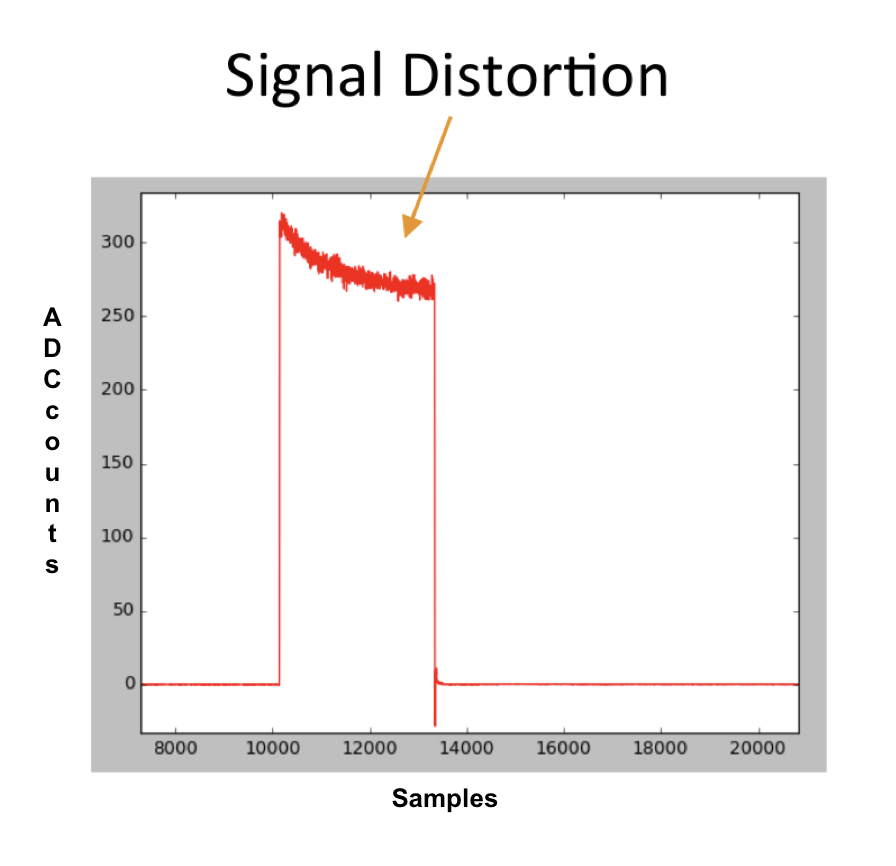
\includegraphics[width=0.4\textwidth]{./figures/5C_base.png}
    \caption{Linearity of the PMT base with 2 stage capacitors (5 units). 80us pulse}
    \label{fig:5C}
  \end{center}
\end{figure}

\par The linearity test bench has been used to optimize the PMT base circuit design (fig. \ref{fig:Base_Sizing}). In order to meet the radiopurity limits \cite{1029-8479} a first proposal based on a minimum of 2 stage coverage (5 capacitors to withstand the high voltage between terminals) has been tested. Although generally this design shows good linearity there remain some long-pulse-length signals with non-linear distortion in time  (figure \ref{fig:5C}). The output signal does not show a typical overload effect which would appear in the case of a usual fall in the gain value for high number of photons. The observed behavior is related to a distortion mechanism that appears due to charge redistribution in the base capacitors. It is possible for a capacitor which has been depleted to drain charge from the capacitor previous to it in the chain. If charge drained by the former is too high, voltage drops accumulate, affecting overall gain. The length of signal pulse able to generate this distortion depends on the time constants of each stage and may change with voltage distribution among stages. The measured linearity  \footnote{Measured as the worst case deviation from the linear fit} for two stage configuration is 1.95\% for 100k photo electrons. This means that a better capacitor coverage is required so a 3 stage configuration is proposed (figure~\ref{fig:7C_layout}). This circuit shows virtually no time distortion. The linearity fit gives a 0.38\% for 140k pe. which exceeds the initial requirements for linearity (less than 1\%).

\begin{figure}
  \begin{center}
    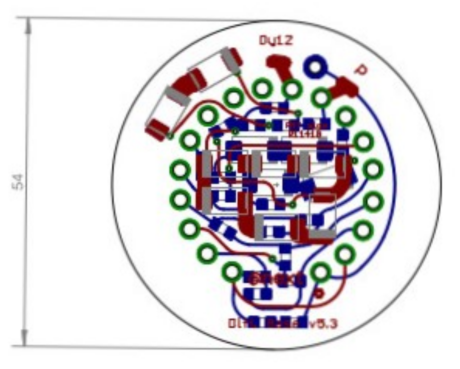
\includegraphics[width=0.45\textwidth]{./figures/7C_layout.pdf}
    \caption{Base Circuit layout}
    \label{fig:7C_layout}
  \end{center}
\end{figure}

\section{Front-end electronics}

\par Front-End Electronics (FEE) and complementary Digital Signal Processing (DSP) techniques will be described in this section. Also data measurements taken in order to verify FEE behavior and validate DSP techniques will be presented. 


\subsection{Grounded cathode connection}

\par The use of an AC coupling scheme implies a high pass filter (HPF) will be created. Such a filter blocks DC component and attenuates frequency components below the cutoff frequency ($f_{cutoff}$). The whole model of FEE includes last stage effect of the base \mbox{((R2 parallel with C1) + R1)} by the pseudodifferential connection. In order to reduce complexity we assume R2 has such a high value that it can be neglected. Figure \ref{fig:GC_equivalent_circuit} shows the electrical equivalent circuit of the connection scheme with a simple current source model as the PMT. The Laplace transfer function of the whole system can be obtained as: (eq. \ref{eq:1})

\begin{equation}
\frac{v_O}{i_I}=A\frac{Z_{in}R_1}{Z_{in}+R_1}\frac{(R_1+Z_{in})Cs}{1+(R_1+Z_{in})Cs}
\label{eq:1}
\end{equation}

\begin{equation}
f_{cutoff}=\frac{1}{(R_1+Z_{in})C_2.2\pi}
\end{equation}


\begin{figure}
	\begin{center}
		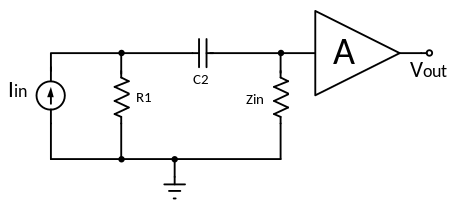
\includegraphics[width=0.3\textwidth]{./figures/FEE_simple.png}
	\end{center}
	\caption{Grounded Cathode Equivalent Circuit and Frequency response}
	\label{fig:GC_equivalent_circuit}
\end{figure}


PMT base capacitors can exchange some charge with the coupling capacitor, so they should be included in the model. Using an equivalent circuit shown in figure~\ref{fig:FEE_PMT} (a) which can be even further simplified (b), the equations shown in eq. \ref{eq:full_fee} arise. Thus the original high pass filter turns into a pole/zero combination as shown in the low frequency range of the final FEE frequency response.

\begin{figure}[!tbp]
	\centering
	\subfloat[FEE + PMT base  ]{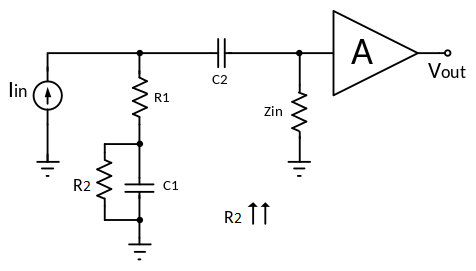
\includegraphics[width=0.3\textwidth]{./figures/FEE_PMT.png}}
	\hfill
	\subfloat[FEE + PMT base  simplified]{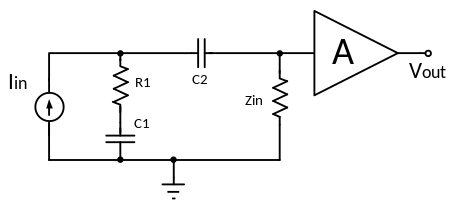
\includegraphics[width=0.3\textwidth]{./figures/FEE_PMT_simple.png}}
	\caption{FEE Full model.}
	\label{fig:FEE_PMT}
\end{figure}

\begin{equation}
\frac{v_O}{i_I} = \frac{Z_{in}}{(1+\frac{C_1}{C_2})}\frac{1+R_1C_1s}{1+\frac{(R_1+Z_{in})C_1}{(1+\frac{C1}{C2})}s} 
\label{eq:full_fee}
\end{equation}


\subsection {High $\tau$ constant value solution}

Since the $\tau$ (time constant) of the equivalent circuit shown in figure \ref{fig:Full_Freq_high_tau} is proportional to the inverse of $f_{cutoff}$, a higher $\tau$ will attenuate a shorter range of frequencies producing a signal which closely resembles the original one. However there is a problem with the implementation of this solution: good quality AC coupling capacitors that can withstand high voltages typically have low nominal values. It is hard to find capacitors higher than $\sim$10~nF that meet such specifications forcing the use of high value resistors. 

Such high value resistors may amplify low frequency components as shown in eq. \ref{eq:full_fee}. This effect will translate into additional baseline shifts or baseline wandering. 

\begin{figure}
	\begin{center}
		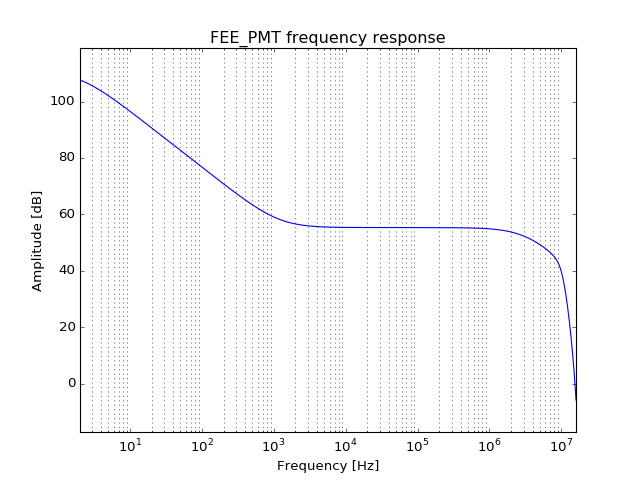
\includegraphics[width=0.4\textwidth]{./figures/tau_badidea.png}
		\caption{FEE Full Frequency Response for high $\tau$ solution.}
		\label{fig:Full_Freq_high_tau}
	\end{center}
\end{figure}

\subsection{Digital Baseline Restoring alternative}

Our proposal for this novel FEE design is to reduce the value of the R1 resistor. This would bring a wide swing in the baseline but it can be accurately recovered using a Digital Signal Processing algorithm once the AC coupled signal has been acquired. The decision has been taken based on the results shown in the previous section: extremely high resistor values gave results too close to the energy resolution limits, and second order effects related to components parasitics might have a strong influence on final results. Moreover high impedance nodes such as the associated to high resistors are more sensitive to coupled external noise. As a result, a trade-off between low frequency effects suppression and feasibility of signal recovery has been established. The lower the $f_{cutoff}$ the easier to recover the AC coupled signal but the higher the vulnerability to low frequency noise and baseline random walks that can have a very negative effect on energy resolution computation in long signals. A value of R1=$1600~\Omega$ has been chosen which gives a $f_{cutoff}$ = 10~kHz. This should attenuate most of the common noises related to electrical engines and other industrial environment elements. Higher $f_{cutoff}$ frequencies would provide a better filtering effect but also would reduce SNR due to the loss in signal amplitude in AC coupled signals.

\par Noise has been one of the most important specifications, carefully studied from the beginning in order to enhance energy resolution results. The active components in the FEE have been chosen mainly relying on their noise specs. The bandwidth of the FEE (3~MHz) has been chosen to make it work as a shaping filter stretching the time length of the single photo-electron (SPE) response. This last aims at improving the sampling operation carried out at the DAQ level due to its sampling frequency limit. However a rise in SPE length introduces an amplitude loss which must be compensated to keep a reasonable signal to noise ratio. This requires a trade-off between SPE length and filter gain.   

% that was provided as a specification by the team in charge of the detector calibration. The SPE must be wider to can measure better with our sampling frequency.

\par   A simplified version of the FEE is shown in figure~\ref{fig:FEE_scheme}. A pseudo-differential transmission has been chosen in order to reduce coupled noise which is expected to be high, since the distance between the FEE rack and the vessel is about 12 m. The AC coupled transmission enables the injection of the high voltage supply to the PMTs through the same signal cable. Assuming C2 AC coupling capacitor has a self resonant frequency (SRF) higher than the maximum estimated bandwidth of the FEE,  the line termination ($120~\Omega$) will be implemented at Zin. This design choice also allows to terminate the common mode signal that travels along the transmission line and is expected to be quite high since a non-fully-differential transmission is being used. The common mode termination is implemented at the amplifier input ($\pi$ type termination with RA and RB).

\par Mirror capacitor C1 acts as base stabilizers in order to further enhance linearity in the PMT, so they should have a value similar to the PMT base capacitors.


\begin{figure}
	\begin{center}
		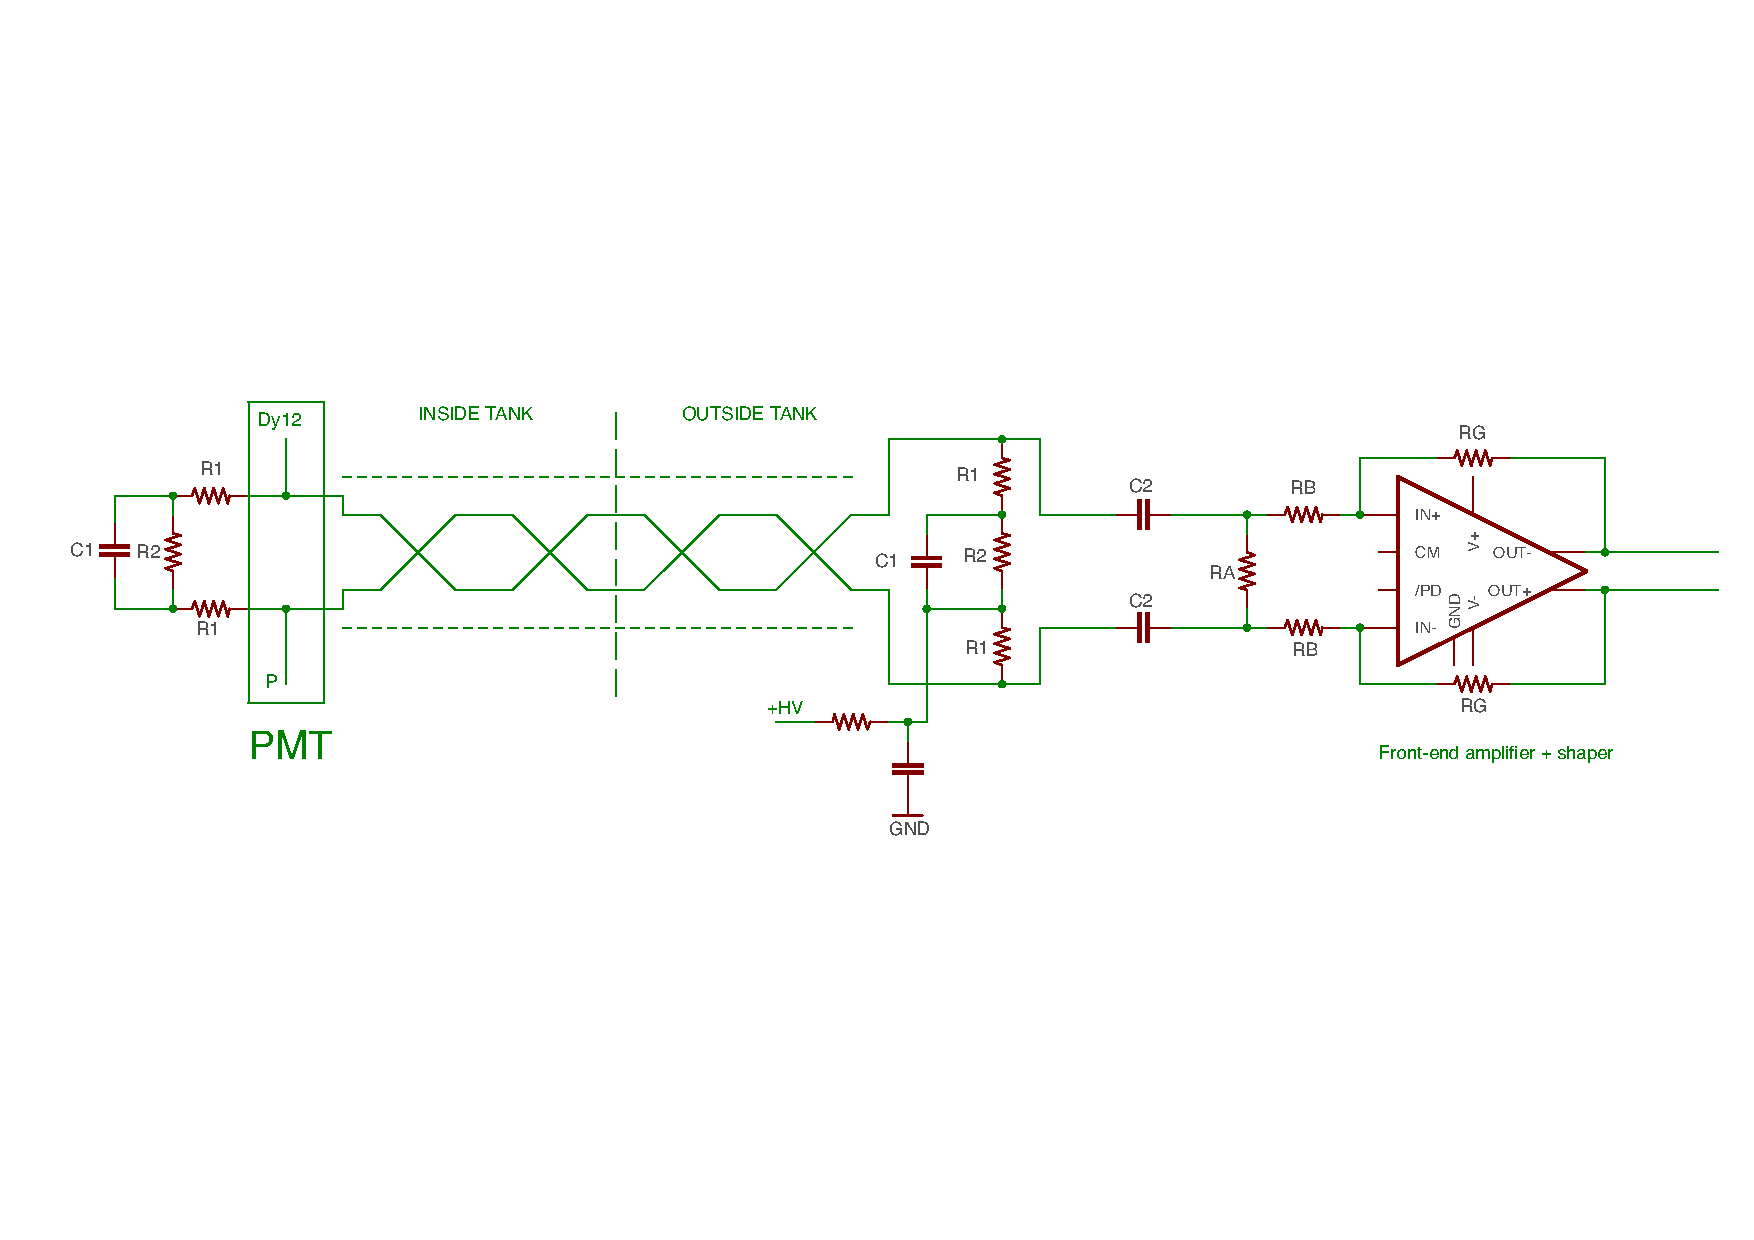
\includegraphics[width=.55\textwidth]{./figures/FEE_simple_scheme.pdf}
		\caption{Simplified FEE Scheme}
		\label{fig:FEE_scheme}
	\end{center}
\end{figure}


\subsection{Noise Measurements}
In order to verify if the design specifications are met, noise measurements carries out both at testbench and at the LSC NEXT installation. The results are shown in the table \ref{tab:noise}. 

\begin{table*}[ht]
	\caption{Noise Measurements (in $LSB_{rms}$)}
	\label{tab:noise}	
	\begin{center}
		\begin{tabular}{ c c || c | c |}
			& & IFIC Laboratory & LSC NEXT \\
			\hline
			\multirow{3}{*}{Direct Measurement} & DAQ Sys. & 0.64 & 0.66\\
			& FEE + ATCA & 0.75 & 0.75\\
			& FEE + ATCA + PMT & 0.76 & 0.8\\
			\hline
			\multirow{2}{*}{Indirect Measurement} & FEE & 0.39 & 0.36\\
			& PMT & 0.12 & 0.28\\
		\end{tabular}
	\end{center}
\end{table*}


Noise specs have been fulfilled with a worst case total noise of 0.8 LSB. The theoretically computed noise of the FEE was 0.35 LSB without power supply contribution. The indirectly measured FEE noise contribution is 0.36 LSB which is really close to specifications. Since the FEE is quite lower than the DAQ system contribution the design has accomplished its main goal. An improvement in noise specs probably would require a new DAQ system design.

\subsection{Front-end electronics model for simulation}
Once the design has been validated through real measurements it is important to build a simulation model which can help in the development of other parts of the project. This time the model has a high level of abstraction in order to be easily integrated with the software analysis modules, Python language with help of Numpy-Scipy libraries. The model comprises two different elements: the low frequency range which has already been developed (eq. \ref{eq:full_fee}) plus a fourth order low pass filter (due to the required shaping) with the right gain factor. The model response has been checked against SPICE simulations of the implemented FEE (figure~\ref{fig:Full_Freq}).

\begin{figure}
	\begin{center}
		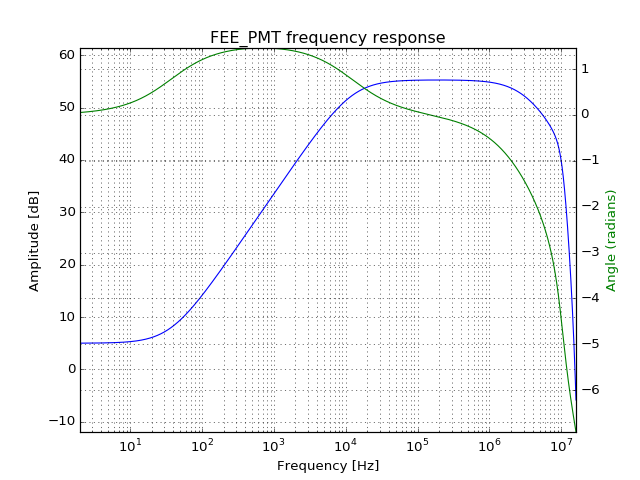
\includegraphics[width=0.4\textwidth]{./figures/FEEfull_freq.png}
		\caption{FEE Full Frequency Response.}
		\label{fig:Full_Freq}
	\end{center}
\end{figure}


Noise generation is introduced in the system to resemble the noise behavior of the real system, taking into account the filtering effect of every part. This is to say that for instance, the input equivalent noise of the FEE has been increased to simulate the observed effect given the 3~MHz bandwidth. The noise equivalent model of the FEE is shown in fig. \ref{fig:noise_eq} as well as the noise equations relative to the different noise contributions:

\begin{align}  
GAIN &= FEE_{GAIN}.DAQ_{GAIN} \\ 
vo_{Tn}^{2} &= v_{DAQn}^{2}(out) + v_{F+Pn}^{2}(out) \\
vo_{Tn}^{2} &= \int_{0}^{BW=3MHz}{v_{F+Pn}^{2}.{\lvert}G.H(jw){\rvert}^2}  \\
& + \int_{0}^{BW=20MHz}{v_{DAQn}^{2}.{\lvert}DAQ_{G}.H(jw){\rvert}^2}\\  
vo_{Tn(rms)} &= \sqrt{vo_{Tn}^{2}} = 0.76LSB_{rms}
\end{align}


Where total Gain is the FEE gain multiplied by adquisition system gain. Moreover, the total noise ($vo_{Tn}^{2}$) is the DAQ out noise ($v_{DAQn}^{2}(out)$) plus the noise of the FEE and the PMT base ($v_{F+Pn}^{2}(out)$).

\begin{figure}
	\begin{center}
		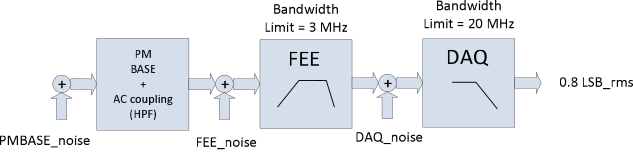
\includegraphics[width=0.5\textwidth]{./figures/NOISE.png}
		\caption{Noise generation scheme}
		\label{fig:noise_eq}
	\end{center}
\end{figure}


\subsection{Digital Baseline Restoration procedure}
\label{Digi_base_res}

\par The design trade-off chosen for this solution allowed a more relaxed FEE design, less prone to low frequency issues and less noisy in general relying on a Digital Signal Postprocessing (DSP) to recover the baseline distortion introduced by the AC coupling capacitor. The DSP algorithm is based on the implementation of a inverse function of a first order high pass filter (HPF). The impulse response of this inverse function has a structure composed of a delta in the origin plus a step function whose amplitude equals the value of $\frac{1}{\tau}$ where $\tau$ is $(R_1+Z_{in}).C$ (eq. \ref{eq:imp}). This means that the convolution operation can be carried out using just an accumulator and a multiplier instead of a FIR filter.

\begin{align}
HPF^{-1}(s)&=1+\frac{1}{\tau.s} \\
HPF^{-1}(t)&=\delta(t)+\frac{1}{\tau} \int_{0}^{t} dt
\label{eq:imp}
\end{align}
   
\par An interesting advantage of this algorithm is that it doesn't have to work continuously, it only has to be activated when a pulse is detected and can be switched off when the pulse ends. This means that an important amount of low frequency noise filtered by the AC coupling capacitor will not be restored since it is slower than the pulse length.

\par However, the low frequency zero introduced by the PMT base interaction adds a low amount of DC to the theoretically AC coupled output signal of the FEE. In order to nullify this effect a high pass filter (cleaning filter) with a cutoff frequency equal to the frequency of this zero is introduced previous to the Digital BaseLine Restoration (DBLR) algorithm. This completely cancels the DC effect so that the reconstructed signal shows no baseline shift at the end. 

\par Since the BLR algorithm uses an accumulator, it might be sensitive to noise and its effects must be studied not only as simple noise equivalent but also taking into account the effect of different frequency components. In case a non zero mean noise appears, the accumulator might get saturated. Typically the accumulator should end the deconvolution process in an empty state, however, the residue low frequency components of the noise makes a small residue remain in the accumulator at the end. Due to finite sampling of the signals residue is not always random. For instance in a burst of short signals (photoelectrons) this residue tends to be positive because the pulses have a higher positive lobe. As a consequence the accumulator starts to rise without limit introducing a baseline shift in the output signal.

\par This novel DBLR algorithm introduces a control based on a smoothing function to deplete the residue remaining in the accumulator after a pulse reconstruction. The algorithm flowchart is shown in figure~\ref{fig:BLR_acc_algor}. In this algorithm the reconstruction process is started independently from the pulse start, and can be working indefinitely. The control relies on the accumulator operations that can be \emph{Update} or \emph{Discharge}. When the DAQ signal rises above a  threshold or the accumulator value is above another threshold (which is the condition for an active pulse) the accumulator is updated as in the original algorithm. However, when none of those conditions are met, which means that there is no active signal pulse, the accumulator is forced to a controlled discharge state. This discharge operation is carried out following a smooth curve so that the reconstructed signal shows no jumps or discontinuities.


\begin{figure}[H]
	\begin{center}
		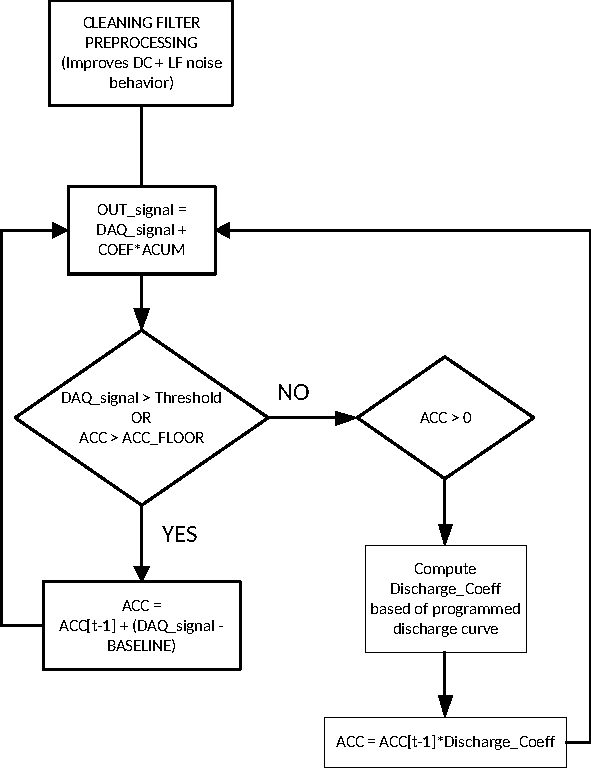
\includegraphics[width=0.4\textwidth]{./figures/BLR_acc_algo.pdf}
		\caption{Accumulator based BLR}
		\label{fig:BLR_acc_algor}
	\end{center}
\end{figure}

\section{Data acquisition system implementation}

\par In the NEXT experiment Data Acquisition System (DAQ), FPGA-based DAQ modules work in free-running mode, storing data continuously in a circular buffer, while an DAQ Trigger module processes trigger candidates received, generating a trigger accept signal that causes data to be sent to a PC farm \cite{1748-0221-11-01-C01008}. Trigger candidates are generated for each PMT channel in the DAQ Data modules, since each PMTs channel is able to sense the primary and/or the secondary scintillation light produced in the chamber. The trigger candidates’ generation is based on the early energy estimation of the events, which requires at the same time a stable baseline \cite{1748-0221-7-12-C12001}. As a consequence digital baseline restoration must be implemented online.

\par A similar version of the DBLR algorithm, introduced in subsection \ref{Digi_base_res} and shown on figure \ref{fig:BLR_acc_algor} has been implemented. This DBLR block is activated whenever the input signal rises above a threshold thus producing an output signal with its baseline completely restored. The threshold  is defined using signal baseline as a reference which requires a precise on-line baseline computation mechanism. A moving average filter has been used in this implementation. In order to avoid baseline shifts due to residues remaining in the accumulator, and further simplify the logic and use of FPGA resources in the DAQ and trigger modules, the control mechanism makes use of a simple linear smoothing function. As in the original algorithm, in case the accumulator is not completely empty when the reconstruction process ends, it must be automatically flushed.

\par The DBLR algorithm has been implemented in a Xilinx Virtex-6 FPGA (XC6VLX240T-1ff1156). There is a DBLR block per channel (12 PMT channels per ATCA-FEC module), and a preceding cleaning filter, both configurable. The implemented algorithm and the cleaning filter have been implemented in a 42-bit fixed point format (Q11.30). The format has been selected as a tradeoff between algorithm stability and physical resources used.


\section{Conclusion}

\par Finally the PMT base was designed and fabricated with the balance between the best possible response and radiopurity. After all the materials involved in the base were screened, we conclude that the level of radiopurity is good for us.  This way we accomplish the radiopurity requirements as well as the electronics requirements.

\par Regarding the front-end electronics, we simulated, designed, manufactured, mounted, tested and we obtained the results that we expected. Once the electronics results were validated as good, we proceeded to build a simulation model. After that, we started with the digital baseline restoration process.

\par The digital baseline reconstruction approach has been designed to reduce front-end electronics complexity thus improving its performance in terms of noise and linearity. Therefore the baseline recovery operation is computed in the digital domain where signal to noise ratio gets hardly affected.

\par Excellent results have been achieved in terms of noise and linearity with acceptable radiopurity levels. Figure 16 shows linearity measurements for the whole front-end including PMT (with its base), FEE and acquisition system. A set of light pulses with constant amplitude and variable length were used.  

\begin{figure}[H]
	\begin{center}
		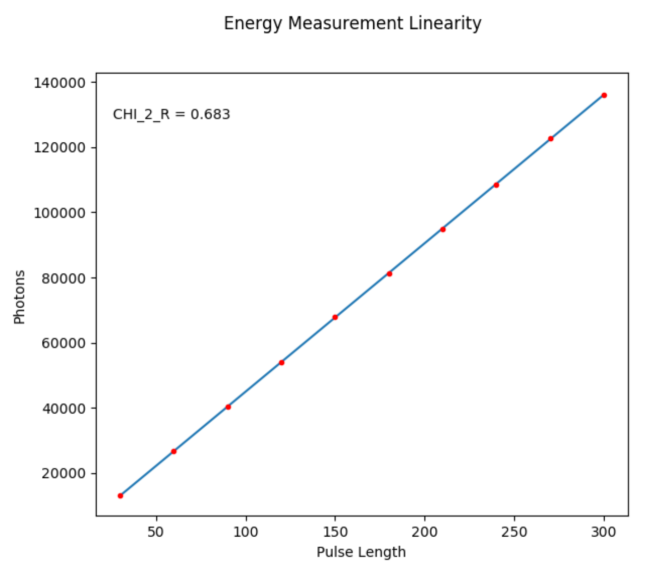
\includegraphics[width=0.4\textwidth]{./figures/7C_lin}
		\caption{Linearity of the NEW base = $0.38\%$ (140kpe)}
		\label{fig:linearity}
	\end{center}
\end{figure}

\par Figure 17 shows a real PMT signal with AC coupling effects (a) and the resulting signal after DBLR has been applied (b) 

\begin{figure}
	\centering
	\subfloat[Blue - Real input signal; Orange - FEE output signal]{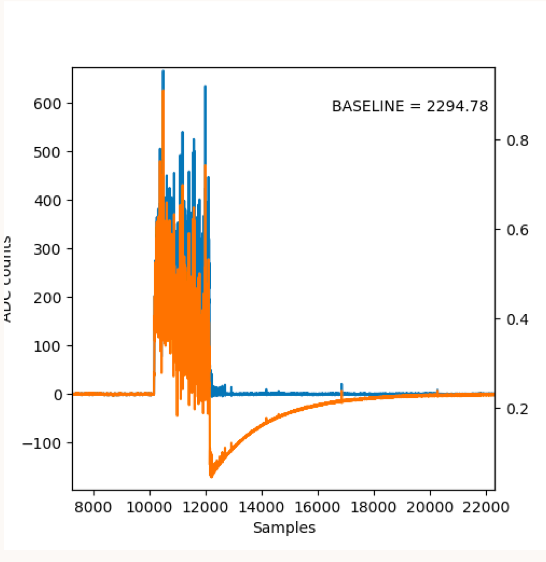
\includegraphics[width=0.4\textwidth]{./figures/signal_preblr}}
	\hfill
	\subfloat[Digital baseline reconstruction applied]{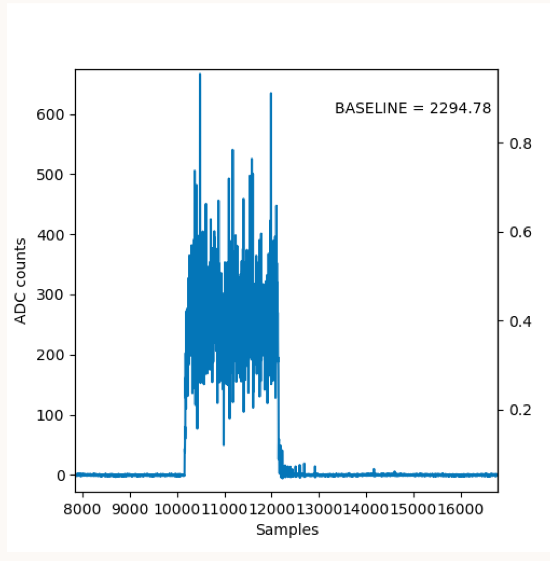
\includegraphics[width=0.4\textwidth]{./figures/signal_blr}}
	\caption{Signal of 50us pulse. 25865 pe. Noise 0.74 LSB}
	\label{fig:graph_sig}
\end{figure} 

\section{Acknowledgments}

The NEXT Collaboration acknowledges support from the following agencies and institutions: the European Research Council (ERC) under the Advanced Grant 339787-NEXT; the Ministerio de Econom\'ia y Competitividad of Spain under grants FIS2014-53371-C04; the GVA of Spain under grant PROMETEO/2016/120; the Portuguese FCT and FEDER through the program COMPETE, project PTDC/FIS/103860/2008; the U.S. Department of Energy under contracts number DE-AC02- 07CH11359 (Fermi National Accelerator Laboratory) and DE-FG02-13ER42020 (Texas A\&M); and the University of Texas at Arlingtonn and special thanks to the Laboratorio subterr\'aneo de Canfranc.


\section*{References}

\bibliography{EP_article}



\end{document}


